\documentclass[11pt]{scrartcl}\usepackage[]{graphicx}\usepackage[]{color}
%% maxwidth is the original width if it is less than linewidth
%% otherwise use linewidth (to make sure the graphics do not exceed the margin)
\makeatletter
\def\maxwidth{ %
  \ifdim\Gin@nat@width>\linewidth
    \linewidth
  \else
    \Gin@nat@width
  \fi
}
\makeatother

\definecolor{fgcolor}{rgb}{0.345, 0.345, 0.345}
\newcommand{\hlnum}[1]{\textcolor[rgb]{0.686,0.059,0.569}{#1}}%
\newcommand{\hlstr}[1]{\textcolor[rgb]{0.192,0.494,0.8}{#1}}%
\newcommand{\hlcom}[1]{\textcolor[rgb]{0.678,0.584,0.686}{\textit{#1}}}%
\newcommand{\hlopt}[1]{\textcolor[rgb]{0,0,0}{#1}}%
\newcommand{\hlstd}[1]{\textcolor[rgb]{0.345,0.345,0.345}{#1}}%
\newcommand{\hlkwa}[1]{\textcolor[rgb]{0.161,0.373,0.58}{\textbf{#1}}}%
\newcommand{\hlkwb}[1]{\textcolor[rgb]{0.69,0.353,0.396}{#1}}%
\newcommand{\hlkwc}[1]{\textcolor[rgb]{0.333,0.667,0.333}{#1}}%
\newcommand{\hlkwd}[1]{\textcolor[rgb]{0.737,0.353,0.396}{\textbf{#1}}}%
\let\hlipl\hlkwb

\usepackage{framed}
\makeatletter
\newenvironment{kframe}{%
 \def\at@end@of@kframe{}%
 \ifinner\ifhmode%
  \def\at@end@of@kframe{\end{minipage}}%
  \begin{minipage}{\columnwidth}%
 \fi\fi%
 \def\FrameCommand##1{\hskip\@totalleftmargin \hskip-\fboxsep
 \colorbox{shadecolor}{##1}\hskip-\fboxsep
     % There is no \\@totalrightmargin, so:
     \hskip-\linewidth \hskip-\@totalleftmargin \hskip\columnwidth}%
 \MakeFramed {\advance\hsize-\width
   \@totalleftmargin\z@ \linewidth\hsize
   \@setminipage}}%
 {\par\unskip\endMakeFramed%
 \at@end@of@kframe}
\makeatother

\definecolor{shadecolor}{rgb}{.97, .97, .97}
\definecolor{messagecolor}{rgb}{0, 0, 0}
\definecolor{warningcolor}{rgb}{1, 0, 1}
\definecolor{errorcolor}{rgb}{1, 0, 0}
\newenvironment{knitrout}{}{} % an empty environment to be redefined in TeX

\usepackage{alltt}

\setlength{\oddsidemargin}{0in}  %left margin position, reference is one inch
\setlength{\textwidth}{6.5in}    %width of text=8.5-1in-1in for margin
\setlength{\topmargin}{-0.5in}    %reference is at 1.5in, -.5in gives a start of about 1in from top
\setlength{\textheight}{9in}     %length of text=11in-1in-1in (top and bot. marg.) 
\linespread{2}

\usepackage{placeins}
\usepackage{setspace} 



\usepackage{amsmath,amssymb}
\usepackage{amsthm}
\usepackage{graphicx}% Include figure files
\usepackage{caption}
\usepackage{color}% Include colors for document elements
\usepackage{dcolumn}% Align table columns on decimal point
\usepackage{bm}% bold math
%\usepackage[numbers,super,comma,sort&comprress]{natbib}
%\usepackage[nolists, nomarkers, figuresfirst]{endfloat}

%\usepackage[american]{babel}
%\usepackage[babel]{csquotes}
\usepackage{natbib}
\bibpunct{(}{)}{;}{a}{}{,}
\renewcommand{\harvardurl}[1]{\textbf{URL:} \url{#1}}

\usepackage{unicode-math}
\unimathsetup{math-style=TeX}
%\setmathfont{Kingfisher-Italic}
%\setmathfont[Digits,Latin,Greek]{Asana Math} 
%\setmathfont[]{Asana Math} 

% font for base text
%\setmainfont[Scale=1.025]{Kingfisher-Regular}

\def\bibindent{\vskip 6pt \hangindent=1 true cm\hangafter=1 \noindent}
\usepackage{hyperref}
\usepackage{xcolor}
\hypersetup{
    colorlinks,
    linkcolor={red!50!black},
    citecolor={blue!50!black},
    urlcolor={blue!80!black}
}

\usepackage{fontspec}
\defaultfontfeatures{Mapping=tex-text}
%\setmainfont[Ligatures=TeX]{CrimsonText-Regular.ttf}
%\setmainfont[Ligatures=TeX]{SourceSansPro-Regular.ttf}
\setmainfont[Ligatures=TeX]{palatino.ttf}
\setmainfont[ItalicFont={Palatino-Italic.ttf}]{palatino.ttf}
\setsansfont{avenir-next-regular.ttf}

\usepackage{caption}
\captionsetup{font={sf,small}}


%\usepackage{sectsty}
%\allsectionsfont{\normalfont\sffamily}

\usepackage{titlesec}
\usepackage{titling}

%\newfontfamily\headingfont[]{Avenir.ttc}
%\newfontfamily\headingfont[]{Myriad.ttf}
\newfontfamily\headingfont[]{Avenir Next.ttc}
\newfontfamily\titlefont[]{avenir-next-regular.ttf}

%\newfontfamily\headingfont[]{avenir-next-regular.ttf}

%\titleformat*{\chapter}{\sansfont}
\titleformat*{\section}{\Large\headingfont}
\titleformat*{\subsection}{\large\headingfont}
\titleformat*{\subsubsection}{\large\headingfont}
\renewcommand{\maketitlehooka}{\headingfont}

\addtokomafont{pagenumber}{\small\titlefont}




\definecolor{background-color}{gray}{0.98}

\newtheorem{theorem}{Theorem} 
\newtheorem{lemma}{Lemma} 
\newtheorem{proposition}{Proposition} 
\newtheorem{corrolary}{Corrolary} 

\usepackage{abstract}
\renewcommand{\abstractnamefont}{\headingfont}
\IfFileExists{upquote.sty}{\usepackage{upquote}}{}
\begin{document}


\title{\titlefont{Partisan Socialization and the Foundations of Stable Partisanship}}

\author{\titlefont{Bradley Spahn}\thanks{Ph.D. Candidate, Stanford University Department of Political Science, \href{mailto:bspahn@stanford.edu}{bspahn@stanford.edu}. A copy of this paper is available from \href{http://stanford.edu/\~bspahn}{bradleyspahn.com}.}}

\date{
\titlefont{\today\\\href{http://stanford.edu/~bspahn/Spahn_Socialization_and_Stability.pdf}{\textcolor{blue}{\\Click here}} for the latest version.
}
}

\begin{singlespacing}
\maketitle
\end{singlespacing}




\begin{abstract}
\singlespacing
After 60 years of partisan stability, large numbers of voters are switching parties. From 2014-2016, 10\% of voters that identified with one party moved to the other two years later. This marks the most rapid switching of party affiliation since the New Deal realignment. To contextualize this partisan volatility, I introduce a new dataset, the California Great Registers, voter lists documenting 57 million voter registrations from 1908 to 1968, matched to census records covering the same period. Before the realignment, party-switching rates were twice contemporary levels; 10\% of voters switched parties every four years. Women and young people, segments of the electorate one would predict to be especially prone to switch, are as stable as the rest of the electorate. This suggests that partisan socialization was weak across the board, which I attribute to the weak relationship betwen group membership and party identification.  The partisan instability early in the twentieth century provided promising conditions for a realignment, which came about in 1932.  Because the recent increase in switching is concentrated among the young, who would be expected to have the weakest attachments, a broad-scale realignment is unlikely in the near future. 
\end{abstract}

\subsection*{Introduction}


Two core elements of our understanding of partisanship, stability and socialization, are deeply entwined. The common explanation for why partisanship is stable is that young people are socialized into a partisan identity, which they hold onto throughout their lives \citep{green2004partisan,ghitza2014great}. The United States experienced rapid partisan realignments in the 1820s, 1860s, 1890s and 1930s, but no such rapid change in the eighty years since the New Deal realignment.  During these periods, voters must have either been more weekly attached to a party or events must have been sufficiently dramatic to overcome any such attachments. In the long period of partisan stability that followed, important events like the Vietnam War, Watergate and the Great Recession were not linked with major partisan realignments, even though the wars and economic calamaties of the past were linked with major changes in the country's partisanship. 

That there has been no rapid partisan change in eighty years does not imply that America's partisan makeup is stagnant. Rather, the slow conversion of Democrats to Republicans during the Southern realignment and the process of generational replacement have driven gradual change in America's partisan composition. These forces are sufficient to produce change in America's partisan makeup, but by their nature, could not drive the kind of rapid shift in partisanship seen in critical realignments. 

It remains a question why critical realignments have become less common. One possibility is contextual: no event has been sufficient to drive major changes in the partisan makeup of the United States. But behavioral changes must also be considered; perhaps Americans have become less willing to change parties in response to events.  Why were such critical realignments more common in the past than they are today and what does that mean for the electorate's ability to respond to major events?

In the latter half of the twentieth century, only about 5\% of voters switched parties every four years, but this long period of post-war partisan stability has recently come to an end. From 2012 to 2017, the Voter Study Group found that 13\% of partisans switched to the opposite party. Similarly, the Pew American Trends Panel found the rate of switching from December 2015 to March 2017 to be 10\%, suggesting that the campaign and election of Donald Trump played an important role in the uptick in partisan instability. Both panels found that young people were much more likely to switch parties than older voters, implying that those who have been most weakly socialized into belonging to a particular party (young people) are also most likely to leave that party. 

This paper proceeds from the observation that the most important tool for understanding partisanship, the scientifically sampled political survey, was developed in 1936, just as the New Deal realignment was ending \citep{norpoth2013polls}. This accident of history, that the period before the realignment was never probed by modern surveys, has left open the question of whether the nature of voters' partisan attachments before the New Deal realignment were similar in stability and structure to after. If partisanship was stable in the 1920s, then the realignment came as a sudden bolt from the blue, unsticking strong partisan attachments that voters had held for decades. If the realignment followed a period of partisan fluidity, then there was less partisan stasis for events to overcome. 

Understanding the circumstances of earlier realignments is vital in assessing the political system's capacity for change. If previous realignments emerged out of a stable partisan environment then it is more likely that such a change could happen again.  But if the realignment instead came from a period of fluidity, then the transition from partisan stability to rapid realignment would be harder to achieve.  The current political moment, in which partisanship is more unstable than at any moment in polling history, lends this question urgency.  

The New Deal realignment marked the largest partisan change of the twentieth century, ending decades of Republican dominance and inaugurating a period of Democratic ascendancy, including sixty years of continuous Democratic control of the House of Representatives. After President Hoover was unable to stop the economic turmoil of the Great Depression, Americans voted Franklin Roosevelt into office, giving him a 17-point higher vote share than Al Smith, the Democratic nominee that lost in a landslide just four years earlier. The stark consequences for Hoover and the Republicans demonstrates the power of a democratic political system to bring about political change when politicians fail to deliver positive economic results. 

%This realignment ushered in many of the cleavages present in contemporary American politics and cemented the Democrats as the party of social spending and the welfare state. Outside of the south, it marked a dramatic change in the fortunes of the Democratic party, bringing about both the presidency of FDR and huge Democratic majorities in Congress. Yet in the over eighty years since the realignment concluded in 1936, no comparably dramatic change in the American party system has taken place. It's hard to say if the American political system would have benefited from a subsequent realignment as sweeping as that of the 1930s, but such a realignment has not transpired. One straightforward barrier to this kind of dramatic partisan change is the stability of individual-level partisanship. From the advent of surveys in the early twentieth century until 2014, it has consistently been found that individuals that identify with one party rarely switch to the other \citep{green2004partisan}.

The extraordinary stability of partisanship in modern times has led to a folk theory of strong partisan socialization. The theory holds that  strong partisan socialization, observed since the beginning of the American National Election Studies, also held in the past. Obviously the theory cannot hold during periods of large-scale partisan change like the New Deal realignment, but when macro-partisanship is stable, it's often held that individual partisanship is also stable. Even during the Southern realginment, overall partisanship was mostly stable, with just a small percentage of voters switching parties each election cycle.

Though this folk theory has not been explicitly characterized before, it pervades important works in political science. In analyzing voting patterns in the American South, Key \citeyearpar{key1949southern} noted that county-level voting in Tennessee was extremely stable in the decades after the Civil War, which he attributed to the "extraordinary durability of voting habits" in the state. That is, he attributed the observed macro-stability in county-level vote shares to individual-level stability. Achen \& Bartels \citeyearpar{achen2016democracy} are even more explicit about the strength of socialization, claiming that not only is partisanship stable, but it is passed on from generation-to-generation, "[Absent realignments], as with religion, people are often adherents of a particular political party because their great-grandparents favored it for entirely different reasons."  In contemporary politics, partisanship is often passed from parent-to-child, but the attribution of this stability to generations that came of age before the New Deal realignment assumes partisan stability in a period before such direct evidence exists. In essence, because individual party affiliations have heretofore been stable, political scientists have assumed that they were stable in the past as well.

The folk theory is also implicit in one of the fundamental theories of American political behavior, Converse's \citeyearpar{converse1966concept} normal vote. The notion that individuals have a stable partisanship that anchors their voting choice is central to the Michigan School's \citeyearpar{campbell1960american} account of political behavior, which puts partisanship at the center of individuals' political attitudes. Given the results available at the time and the decades of evidence that followed, it is reasonable to believe that stable partisanship is an essential and timeless fact of the American political system. Indeed, no evidence has pointed to the contrary.


This paper shows that before the New Deal realignment, individual partisanship was characterized by instability, even while overall partisanship was largely stable. 10\% of major party voters switched to the other party every four years, a rate higher than has been observed in any ANES panel study. This instability was widespread and not concentrated among particular age or demographic groups, suggesting that party attachments before the realignment are not compatible with a theory of widespread partisan socialization. 

The failure of the folk theory of partisan socialization  to explain partisanship before the New Deal suggests that partisan socialization is not a fundamental feature of the American political system. Rather, socialization emerged as a phenomenon when the country was in considerable economic upheaval and government intervention in the economy increased dramatically. Federal government spending tripled during the Great Depression, while at the same time, voters' attachments to the parties greatly increased. It's impossible to determine what precisely drove the change from the partisan instability of the 1910s and 1920s to the partisan stability that followed the New Deal realignment, too much was changing all at once to tease out the causal threads. But one can confidently declare from the evidence provided by the Great Registers that partisan stability is context-dependent.

Lipset \& Rokkan \citeyearpar{lipset1967cleavage} note the party cleavages of several countries, including the United States, froze around political competition between the political interests of the owners of capital and those of labor. This realignment finished in the United States in 1936. That the freezing of partisan identities  and the freezing of the core cleavage defining the (non-Southern) American party system both occured in 1936 leaves open the possibility of a causal link. The coincidence of these two political phenomena suggests that the longevity of America's fifth party system may not be attributable only to the issue orientation of the two parties, but also to the strength of the partisan attachments of their voters.

I'll begin by introducing the California Great Registers in more detail and describing the cross-sectional partisan composition of the electorate from 1908 to 1930. The rest of the paper will focus on party switching. First, I'll demonstrate that party-switching rates from 1908 to 1928 were considerably higher than in the latter half of the twentieth century, which is an indication that partisan socialization may be weaker in the period. I go on to examine whether newer voters, who should be more weakly socialized into a party, making comparisons with post-war and contemporary switching rates to show how partisan socialization has strengthened over time. Finally, I'll discuss the implications of today's pattern of party-switching for the prospects of a future realignment. 


\subsection*{Data \& Methodology}

Lamenting the lack of data suitable for studying long-term partisan change, V.O. Key \citeyearpar{key1959secular} wrote, "The ideal data for this purpose would consist of political life histories, extending over several generations, of random samples of population categories. Until such data miraculously become available, the only alterative is to search out electoral areas in which specific kinds of people are concentrated and to analyze the voting behavior through time of the people of such areas."

Ironically, such representative panel data already existed when Key wrote his 1959 article. Spread over 735 thousand pages in over 600 volumes, the California Great Registers, the collected voter lists of every California county, chronicle the partisanship of every California voter from 1900 to 1944, and in some counties, even later.  The Registers include the name, address, party registration and, in most cases, occupation, of every Californian registered to vote during the period. California had closed primaries starting in 1910, which incentivized voters to register with a major party, since unaffilated and minor party members could not vote on the major parties' nominees.   From 1910-1932, voters re-registered each election year, requiring that voters file a new registration before each general election to vote. 

%After the passage of Proposition 14 in 1930, this requirement was relaxed. Beginning in 1934, registrations from the last election remained active so long as a ballot was cast in either a primary or general election during the previous two-year cycle. If a registrant didn't vote, as was the case for about 20\% of voters registered in presidential years and between 25\% and 40\% in midterm years, they would receive a notice indicating that they would need to re-register to vote in the next election.  This process of bi-annual re-registration before 1934, and less frequently thereafter, provided the Registers with a regular update on the partisan attachments of California's electorate. Because they cover every county of a populous and diverse state, the Registers capture the political behavior of a broad range of people with individual-level data updated every two years.

The Great Registers were typeset by the counties, printed, bound, and deposited in the California State Libary in Sacramento. They have proved valuable to genealogical researchers because they provided an expansive (though not exhaustive) listing of Californians' name, address and occupation. Genealogists use the Registers to track the movements of their family members and to provide a connection to the past.  Archival records have increasingly become digitized, making genealogical research more accessible and more efficient.  Ancestry.com, a  commercial platform for genealogical research, digitized and performed optical character recognition (OCR) on the registers, parsing the digitized text into name, gender, address, party and occupation fields. For Ancestry customers, this parsing allows individual names and addresses to be searched and located in the Registers.  For research purposes, they provided a large tabular dataset that can be analyzed at scale, without needing to refer to the original printed page.  

Some counties, especially rural counties, archived many years worth of voter registers into a single book. When this data was scanned by Ancestry.com, data on the specific year to which a particular voter registration refers was lost. In Kern County, for example, the Great Registers for 1900-1910 were all bound together, making it impossible to assign specific voter registrations to specific years. Because all of the analysis in this paper involve following a measurement across time, Great Register volumes that cover more than one presidential election are dropped from the analysis.  This means that the Kern records for 1900-1910 and 1924-1932 are dropped, but the 1920-1922 book is included in the analysis, with all of the registrations assigned to the presidential year, 1920. Since this archiving issue only affects smaller counties, such records comprise a small part of the overall dataset. 


%Transcription errors in the data are common but can often be resolved through fuzzy text-matching, whereby text strings that don't match exactly to known good values can be matched to their closest match, and corrected in the original data.  For instance, ``housewife'' is by far the most common occupation in the Registers, but the string ``housewif'' appears frequently as well.  Since ``housewif'' would not match to a list of proper occupations, fuzzy string matching would return a match to ``housewife,'' and the error would be corrected. The same process can be applied to names and street names to clean up transcription errors that appear in the data. Sometimes, unsual strings that were nonetheless digitized correctly will be improperly corrected. For instance, an unusual name like ``Geoffry'' might be corrected to ``Geoffrey,'' even if the man's actual name is ``Geoffry.'' In these cases, the name will reliably be changed to its more common variant, so that no information is lost.

One important distinction to make in discussing partisan stability is the difference between macro-stability and micro-stability.  Macro-partisan stability is easily observable from cross-sectional data. If one looks at candidate vote totals or party registration shares year-by-year, one can infer how partisanship in the overall electorate is changing.  From 1920 to 1930, for instance, overall support for Republicans increased in California. While it's likely the case that the Republican party's ranks grew from 1920 to 1930, one can't readily infer from cross-sectional data whether these gains were characterized by large numbers of people moving between the parties (with most of one party's losses offset by new registrants from the other), or instead by high levels of stability, with just a few members switching parties. Panel data, on the other hand, would tell us what the overall rate of instability would be by comparing individuals' party affiliations in 1920 to their party affiliation in 1930.

Voters' registration records can be matched to their own records in successive years, creating a panel dataset for the tracking of partisan change over time.  For instance, each appearance of Ronald Reagan at 1669 San Onofre Dr. would be linked, so that his partisanship can be followed from election to election. In this way, a measure of the quadrennial change in a voter's party registration can be constructed for all voters for all the years covered by the dataset.  For the purposes of constructing panel data for this paper, first names, surnames and street names were matched to the most similar string known to be correct with an edit distance less than four. So, for instance, "fiflh" street would be corrected to "fifth" street. After this correction was applied, I matched records from one year to the other on full name and address. This matching method is very conservative, matching about 7\% of records to a record four years later. This conservative procedure keeps the rate of false-positive matches to a minimum, minimizing any inflation of the party-switching rate due to erroneously matching one person to another.

Recent advances in computation have made probabilistic record linkage easier, but significant challenges remain in linking data of this size.  McVeigh, Murray \& Spahn \citeyearpar{mcveigh2018scaling} develop a bayesian probabilistic record linkage algorithm for linking the 1932 and 1936 Alameda County registers, which is itself the largest dataset to be linked using bayesian techniques. Each of these registers contain about 250,000 records, orders of magnitude fewer records than are present in the full dataset. Even at this smaller scale, computation is extremely difficult, talking about 2 days to complete. Computationally cheaper non-bayesian procedures are available for record linkage, but McVeigh et al show that these perform poorly on the Great Registers, because the frequent transcription errors make separating the matching and non-matching cases difficult. Luckily, McVeigh et al's preferred record linkage algorithm, which they refer to as "strict," recovers the same match rate as the exact-matching algorithm described above. Though the Bayesian algorithm finds about 50\% more matches, these additional matches don't change the point estimate of the party-switching rate. Further, the algorithm uncovers very little uncertainty in the linkages, about a third the magnitude of the frequentist sampling variability  for the same data. Given these results, the exact matching procedure can be reasonably substituted for a probabilistic record linkage algorithm without significant concerns about the validity of the results relative to other matching procedures.


A shortcoming of the registry data is that it lacks the kinds of demographic information that would be available on a survey.  Luckily, individually-identified U.S. census data is released 72 years after the decennial census was conducted, meaning that the 1920, 1930 and 1940 censuses are available at the individually-identified level.  I matched these censuses to the Great Registers, allowing the full set of census covariates to be analyzed together with individual-level party registration data. Together, this amounts to a 57-million record panel dataset attached to a population-level census providing detailed demographic, economic and housing data for millions of Californians, spanning the period 1908 to 1944.

Though this paper compares trends in California with trends in the broader United States, one set of states that California should not be compared to is the South. Southern states did not realign toward the Republicans in 1894, instead remaining consistently supportive of the Southern Democratic party, in contrast to Republican dominance in California. Southern voters also had lower rates of turnout. The voter turnout rate was only about a quarter in the Southern states, compared to just under half for the rest of the country \citep{burnham1965changing}. The implications of using California to investigate early 20th century political behavior more broadly are discussed in the appendix.

The scope of this paper is broad: it tries to describe 20 years of American politics as experienced by millions of registered voters in California and compare it to canonical results in politial behavior after the realignment. Economy requires that only a limited number of results be offered, and that these results be interpreted in only a limited number of ways, with an aim to advance the argument of this paper: that partisanship before the realignment was considerably more fluid than partisanship post-realignment. These same results could be understood in other ways, contributing to other arguments. 

% Take this out: these same results could be understood in other ways, contributing to other arguments. 


One obvious area of study is the realignment itself.  Indeed, studying politics before and after the realignment, while ignoring the realignment itself, may seem odd. For the sake of narrative economy, the dynamics of the realignment will be set aside for a fuller treatment in other work \citep{spahn2018before}.

For the most part, results will consist of simple proportions, usually of the party-switching rate, either among partisans or all voters, for various subgroups by year. As with any measurement, these proportions are subject to uncertainty, but sampling variability plays a small role here. For one, the Registers are official records: they represent a complete listing of the eligible voters for each election. Some records are lost to transcription errors and bad scans, but this is a minority of cases and happens randomly, a result of an imperfect technological process rather than through some mechanism associated with voter behavior. The records that are left are large in number, so much so that even deep cuts of the data usually have enough elements that sampling variablility is small relative to the comparisons being made. 



% are independents just an intermediate category?
% Look at how big a share progressives got: shows prima facie that party attachments are weak




\subsection*{Two-Party Consolidation}

Though Republicans were the dominant party in California before New Deal, the influence of the Progressive party is unmistakable. Hiram Johnson was elected governor of California as a Republican in 1910, but went on to co-found the Progressive party with Theodore Roosevelt in 1912, serving as its Vice-Presidential nominee in that year.  When Johnson ran for re-election as governor in 1914, the Progressive party made huge gains in voter registration, taking about a quarter of Republican registrants and making them, for a time, Progressives.

Figure~\ref{fig:consolidation} shows that this swell of Progressive affiliation did not last, however.  The Progressives did not field a candidate in the 1918 gubernatorial election, and over time, the party lost nearly all of its registrants.  Though the Socialist and Prohibition parties never received the ground-swell of support that the Progressives received in 1912 and 1914, they too saw their numbers decline to a negligible level by 1920.  By 1922, the rate of voters declining to affiliate with a major party also declined, leading to an increasing proportion of voters registering with the two parties.  By 1930, the last year before the New Deal realignment took place in California, 93\% of voters were registered with one of the two major parties, a rate that declined further in the coming years.



\begin{knitrout}
\definecolor{shadecolor}{rgb}{0.969, 0.969, 0.969}\color{fgcolor}\begin{figure}

{\centering 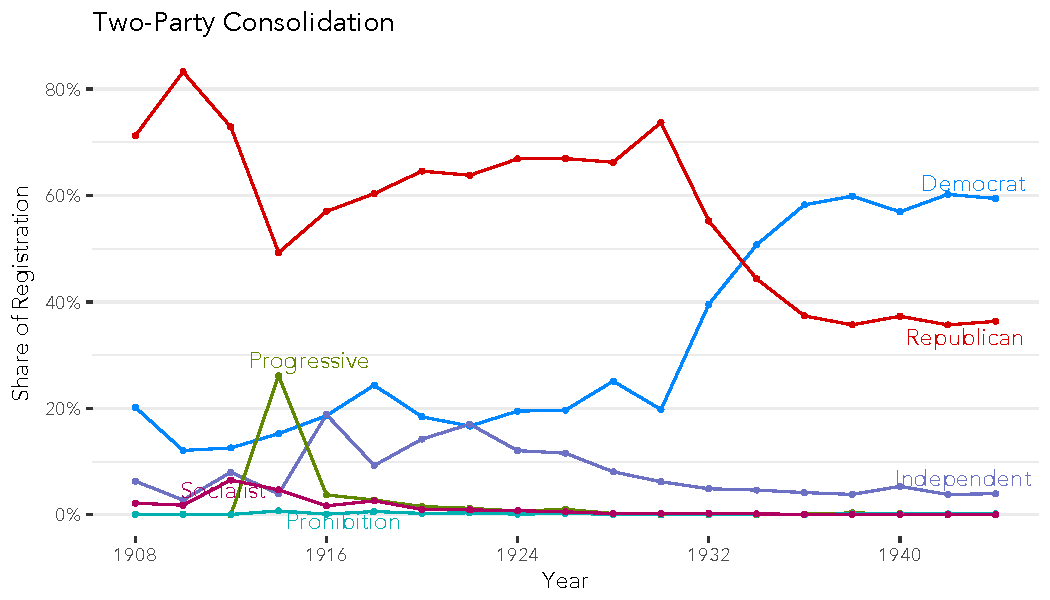
\includegraphics[width=\maxwidth]{figures/plots-consolidation-1} 

}

\caption[Rates of party registration for the most common parties, 1908-1930]{Rates of party registration for the most common parties, 1908-1930. The Socialist and Prohibition party members have been aggregated together with independents into the category, "Other" category. The vast majority of such registrants were listed as independents.}\label{fig:consolidation}
\end{figure}


\end{knitrout}

The high proportion of voters that registered with the two parties is helpful for measuring partisan sentiments.  On the 2013 California voter file, only 72\% of Californias registered with one of the two major parties. Many of the remaining voters themselves held strong partisan preferences toward one party or the other, but this preference is unknowable from voter file data alone. Luckily, many more voters on the Great Registers are affiliated with a party.  Except for 1914, when the shift in party registrations to the Progressives led 30\% of California voters to be affiliated with the Progressive party, the two major parties' share of registrations never dipped below 75\%.  By 1928, the last presidential election before the realignment, just 10\% of the electorate wasn't registered with one of the two parties.



\subsection*{Party Switching}


%%% show that panel data partisanship looks like overall partisanship

That partisanship is stable and central to a voter's political attitudes has been fundamental to the study of American political behavior since the publication of the \emph{The American Voter} in 1960. The simple descriptive fact that voters tend to form a party identity early in their lives and retain it for many years has been measured repeatedly and confirmed to be a consistent feature of American public opinion since the 1950s \citep{green1994stable, clarke2009dynamics}. 




%One early survey item aimed at understanding the degree of partisan stability came from the 1956 National Election Study. The survey asked whether the respondent had ever identified with a party other than their current party. Amongst the respondents that identified with one of the major parties, 15\% reported having ever identified with the other party. This includes people that changed party affiliations during the New Deal realignment, which surely inflated the rate of party-switchers above the level we might expect to observe today, now that we are further from major political realignments.

Though the Literary Digest Straw Polls suggest that presidential vote choice was more fluid before the New Deal realignment, no direct evidence on partisanship is available from survey data before 1936  \citep{erikson1981partisan}. This makes the Great Registers the only viable way to test whether partisanship was stable during the fourth party system, as it is now in the fifth. On this point, the Registers are clear. It was not.

One straightforward piece of evidence that party attachments were weak before the realignment is the rapid rise and fall of the Progressives during Hiram Johnson's campaign for governor in 1914.  The Progressive share of registration rose to almost 30\% in 1914, only to crater two years later.  For these voters, the particular appeal of Johnson was enough to overcome any attachments they had to the Republican party. They moved in spite of the fact that none of the other major offices featured close primaries and Johnson himself ran unopposed in the primary. That is, they didn't move for instrumental reasons. Rather, they wished to express support for the party by registering as Progressive. This interpretation of party registrations as an expressive act is corroborated by contemporaneous newspaper accounts, which interpreted party registration rates as an indicator of the level of support for each party in the state.   After Johnson failed to foster a progressive wave down-ballot, these new Progressives left the party nearly as quickly as they joined, with most Progressive registrants leaving the party by 1916.

Figure~\ref{fig:pid_switching} shows the quadrennial party-switching rate from 1908 to 1928. About 10\% of partisans switched from one party to the other in consecutive  Presidential elections in each of these five cycles.  While one or two cycles of higher party-switching rates could be a fluke, the Great Registers reveal that in California during this period, party-switching rates were consistently  about twice the post-war average. This is true even though the population being studied in this subset of California registrants, people who registered to vote in consecutive Presidential elections and who did not change address, were more politically stable than the population as a whole.




\begin{knitrout}
\definecolor{shadecolor}{rgb}{0.969, 0.969, 0.969}\color{fgcolor}\begin{figure}

{\centering 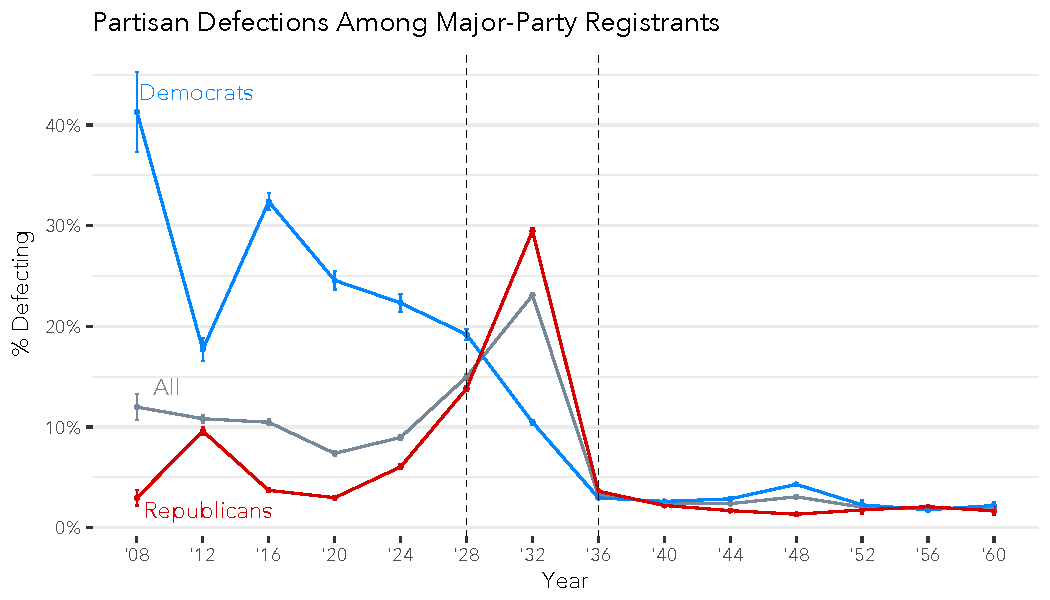
\includegraphics[width=\maxwidth]{figures/plots-pid_switching-1} 

}

\caption[Rates of party switching between successive presidential elections among voters registered with the two major parties in both elections]{Rates of party switching between successive presidential elections among voters registered with the two major parties in both elections. The year on the x-axis refers to the earlier year in the panel. So that the left-most points refer to the percentage of each group switching to the other from 1908 to 1912. The figure was generated by matching records appearing in successive presidential years that share an address, surname, and first name. This stringent requirement for matching excludes movers and records with transcription errors, but keeps false matches, which inflate the rate of party-switching, to a minimum. Frequentist 95\% confidence intervals are plotted as vertical lines.}\label{fig:pid_switching}
\end{figure}


\end{knitrout}
 

Matching over a longer period of time and relaxing the restriction that voters must maintain the same address shows that the rate of party switching is by some measures higher than the 10\% rate shown in figure~\ref{fig:pid_switching}. I began by exact-matching the 1920 and 1930 censuses to the Great Registers from the corresponding year on name and address. Because the 1920 and 1930 censuses contain stable covariates that aren't included on the Great Registers, one can confidently match between subsequent censuses without requiring that matching cases share an address.  I matched the 1920 and 1930 censuses on full name, age, county, city, the respondent's birthplace and the birthplace of their parents. 16\% of major-party registrants switched to the other party ten years later. That the ten-year switching rate is higher than the four-year switching rate shows that most voters change parties and then remain with their new party, rather than quickly switching back. This pattern is consistent with voters switching parties for substantive reasons, rather than simply choosing a party at random, only to randomly switch back later on.

The party-switching rate before 1930 is considerably higher than at any time in the latter half of the twentieth century. On the 1965-1973 Youth-Parent Socialization Panel Study \citep{jennings1981youth}, a group of parents  were interviewed about politics in 1965 and again in 1973; the proportion of parents that identified as partisans in both panel waves who switched from one party to the other was 6\%.  Similarly, in both the 1972-1976 and 1992-1996 ANES panel studies, respondents that identified as a Democrat or Republican in both waves of the panels switched from one major party to the other about 5\% of the time.  The correspondence between the post-1936 Great Registers and survey data is considered in the "The Registers Show Stability After 1936" section of the appendix.

One question to consider is how independents are treated in the analysis.  The number of independents among California voters varied substantially, from less than 5\% in 1910 to over 20\% of registered voters in 1916, yet despite this substantial variation in the role of independents in the electorate, there was very little variation in the party switching rate. If people that sometimes register as independents or with a third party have especially weak partisan attachments, then one would expect a negative correlation between the number of independents and the party-switching rate. But in fact the switching rate is quite stable.  To make a direct comparison, in both the 1916 Great Regiseters and the 1972 ANES, about 20\% of voters didn't identify as members of either party, but from 1916 to 1920, the party-switching rate was 10\%, while from 1972 to 1976, the party-switching rate was half that. Thus the unusually high rate of switching before the realignment can't be attributed to the number of independents at the time.

In some sense these survey measures are incompatible: partisanship from the Great Registers is a measure of party registration, while partisanship from these panel surveys comes from the classic party identification survey question. These two measures are not as different as they might appear. California's voter registration affadavit invited registrants to "affiliate" with a party, calling to mind party membership. This is not unlike the ANES party identification question, which asks respondents whether they think of themselves as Democrats, Republicans or something else. Further, because voters had to register anew for each election, they are expressing their partisan preference without reference to their previous partisanship, just as a respondent does on a panel survey. Finally, county-level presidential vote correlates closely with county-level partisanship, as one would expect from a genuine measure of partisan preference.\footnote{The relationship between county-level Presidential vote share and county-level registration share is discussed further in the appendix section "Is party registration a substitute for party affilation?"}


It might seem that contemporary party registration,  rather than party identification might be the better analogue for party affiliation on the Great Registers, but California's registration laws early in the century are too different than the current laws of any state. No state requires voters who vote and remain at their address to re-register, making any appearance of continuity in party registration an artifact of the registration process. People that move often have to re-register, but moving is often related to other major life changes, which further confounds the comparison.  

One final concern is that voters were registering strategically, rather than expressively. Before 1930, Democratic candidates were mostly not competitive in California. Since California had closed primaries, the only way to influence the selection of the Republican candidate, who usually went on to win office, was to register with the Republicans. Thus, voters might strategically choose to register with the Republican party, even though their loyalties lay with the Democrats.  Primary turnout varied from year-to-year, but it typically stood at about a third of general election turnout, indicating that only a minority of voters were interested enough in politics to cast a ballot in the primaries. The further level of political interest required for Democratic voters to register strategically with the Republicans, in anticipation of voicing primary support for a candidate they would go on to vote against in the general election, was probably rare.

It would obviously be preferable to have the same question asked before and after the realignment,  but since it is impossible to re-survey voters in the pre or post realignment era, we must make the best inferences possible using available data from the Great Registers.




\FloatBarrier

%\subsection{Party Membership}

%Before 1928, the Democratic party, already small, hemoraged an average of 23\% of their voters to the Republicans each election cycle. Figure~\ref{fig:pid_switching} shows the rates at which each party lost their members to the opposing party in successive presidential election years from 1908 to 1928, among members registered with the two parties in both elections. The Democratic party held on to a relatively small proportion of its members through this period, losing around  20\% of its membership to the Republicans in each year from 1908 to 1924 (meaning they appeared as members of the other party from 1912 to 1928). Despite the fact that Democrats had already incurred huge losses in the 1896 realignment, the party continued to lose members until the New Deal realignment began in 1932.  The only reason the Democratic party membership did not shrink further is that these relatively large losses by Democrats were offset by proportionally smaller losses from the Republicans. Because the Republicans had a much larger base to begin with, the Republicans could lose an average of just 5.5\% of their voters to the Democrats each year and have those losses offset by defecting Democrats, who on two occasions lost more than 30\% of their members in a single presidential election cycle.

%This pattern of partisan churn implies something extraordinary about the composition of the Democratic party during the pre-realignment period: a significant proportion of Democrats had recently been Republicans. Figure~\ref{fig:party_composition} shows that in 1916, nearly 30\% of Democrats were registered Republicans four years prior. Political scientists have come to view parties as coalitions of voters, led by political elites, that compete for votes. But if these elites are leading an ever-shifting group of voters, as many as 30\% of whom were recently registered with the opposing party, this model cannot describe partisan competition in the mass public. 

%This disconnect between the partisanship of office-holders, who rarely switched between the two major parties, and voters, who did so frequently, might be explained by the kinds of issues contested in the fourth party system. Aside from prohibition and women's enfranchisement, two issues which drew much fervor but were not polarized along partisan lines, many of the partisan issues of the day were technocratic in nature. Debates about how to handle railroad and industrial trusts, the proper levels of tariffs, the banking system and the gold standard were quite disconnected from the lives of most Americans, particularly relative to the politics of the New Deal, which focused on jobs and public assistance programs during the Depression. As the issues attached to the two parties' platforms became more salient to voters, their attachments stabilized, and the weak attachments of the fourth party system gave way to the strong partisan ties of the fifth party system, which remain today.




 

%The high level of churn in both parties, but especially among the Democrats, must have posed tremendous challenges for party governance. How could party elites form a stable hold over their state parties if so much of the membership turned over every four years? For Democrats before 1936, at least 12.5\% of their members were recently Republicans in each election year, and nearly 25\% of their members were previously Republicans or not registered with a major party in the last election (this doesn't count those members who were not registered at all). One possibility is that primary voters were loyal to their party, while the voters most likely to switch parties did not vote in primaries.  Without turnout data, this is impossible to know, but it seems that a full account of how parties operate during the period must account for the transience in the Democrats' ranks. The GOP's membership was more stable, but the party rolls were filled with fewer stable Republicans than after the realignment, when both parties membership rolls stabilized at less than 5\% churn per year.

\subsection*{Unstable Partisanship and Implications for Socialization}

The preceding section showeds that rates of party switching were considerably higher before the New Deal realignment. This fact requires a re-evaluation of the folk theory of partisan socialization. The most widely-accepted account of partisan stability is that young people are socialized into having a particular party affiliation by their parents and social environment early in life, and that these attachments persist and strengthen into adulthood.  It follows that certain groups who have experienced less partisan socialization should be less stable in their partisanship.  Though Green et al \citeyearpar{green2004partisan} note that heterogeneities in partisan stability haven't been observed in the literature, this can be attributable to the few party-switching cases available in twentieth-century post-war panels.   With the Great Registers matched to census data from the same period, sample size become less of a concern and heterogeneities in stability should be easier to observe.

A core element of partisan socialization is habituation: the theory predicts that those that have supported a party for longer would be more strongly socialized into supporting that party. Thus, the more time a person has been actively supporting one party or the other, say by voting for the party's candidates or registering as a member of the party, the stronger the individual's attachment should be.  The most straightforward way that voters might expect to vary in the strength of their habituation is in the length of their voting history; more experienced voters should be more habituated to supporting a particular party, and thus be more stable in their party registration.  


California enfranchised women in 1911, allowing women to vote for the first time in 1912. The entry of women into the electorate is not merely remembered as a victory for the Suffragists, it's also seen as a contributor to the New Deal realignment \citep{corder2016counting, andersen1979creation}. To explain the massive increase in the political success of Democrats during the New Deal realignment, Andersen suggests that new entrants to the electorate, especially women and immigrants, became politically active during a period very favorable to Democrats, and as such, were more likely to be socialized by their social environment to favor the Democratic party. Implicit in this theory is the idea that women, who as a group were newer to voting than men, were more effected by the dynamics of the current political environment. This provides us with a clear prediction to test: women, who were newer to voting than men, should change their party registration more often. The difference should be especially pronounced in 1912, when California women were allowed to vote for the first time, while men had the opportunity to vote their whole adult lives.







\begin{knitrout}
\definecolor{shadecolor}{rgb}{0.969, 0.969, 0.969}\color{fgcolor}\begin{kframe}


{\ttfamily\noindent\bfseries\color{errorcolor}{\#\# Error in readChar(con, 5L, useBytes = TRUE): cannot open the connection}}

{\ttfamily\noindent\bfseries\color{errorcolor}{\#\# Error in stri\_length(string): object 'plot.df.panelchange.by.sex' not found}}

{\ttfamily\noindent\bfseries\color{errorcolor}{\#\# Error in plot.df.panelchange.by.sex\$source <- "{}Great Registers"{}: object 'plot.df.panelchange.by.sex' not found}}

{\ttfamily\noindent\bfseries\color{errorcolor}{\#\# Error in eval(expr, envir, enclos): object 'plot.df.panelchange.by.sex' not found}}

{\ttfamily\noindent\bfseries\color{errorcolor}{\#\# Error in eval(expr, envir, enclos): object 'plot.df.panelchange.by.sex' not found}}\end{kframe}
\end{knitrout}

Figure ~\ref{fig:switching_by_gender} shows the party switching rates for men and women. They are virtually identical. All of men's accrued experience registering and voting for a party did not increase their partisan stability relative to women. Though women surely read about and discussed politics before they won the right to vote, they weren't allowed to express their preferences at the ballot box.

The extraordinary closeness of the party-switching rates of men and women brings into question the role of early socialization in forming stable partisan attachments.  It's likely that parents would invest less time teaching their daughters about politics than their sons, as would teachers and political institutions, as they wouldn't expect those girls to grow up to vote (or might be less likely to do so than young boys). 

Andersen's \citeyearpar{andersen1979creation} mobilization account of the New Deal realignment rests in part on the expectation that men, who have more experience voting, would be immunized against the partisan tides of the 1930s, while women and immigrants, groups newer to voting, would not be.  But the experience of women in California from 1912 to 1928 suggests that women were no more immunized to partisan tides than men. Both men and women switched parties frequently, bearing none of the partisan stability that the folk theory would predict.

Another way in which partisan habituation varies is in age. Younger voters are necessarily less experienced than their older counterparts, and thus have had less time to became habituated to voting for one party or the other. Thus, I can compare the differences in party-switching between age groups during different periods to understand how partisan socialization varies across time.

I'll consider three periods: the pre-realignment period, which has been treated at length in this paper, the post-war period of partisan stability and the recent period of increased party switching. For the pre-realignment period, the only available panel data comes from the Great Registers matched to the 1920 and 1930 censuses (the censuses provides a source for age, which is unavailable on the Great Registers). 16\% of voters had a different party in 1920 than in 1930.  For the post-war period, I use two ANES panel studies, the 1972-1976 panel and the 1992-1996 panel. Both showed overall switching rates of about 5\%.  For the current period, I use data from Wave 1 (March 2014) and Wave 23 (December 2016) of the Pew American Trends Panel. On a weighted basis, 10\% of panelists switched parties in that period.  Note that while the Great Registers only included registered voters, the others survey the U.S. adult population (in the case of the ANES, the adult citizen population).

The data for 1992-1996 in figure~\ref{fig:switching_by_age} summarizes what political scientists have seen for most of the last 70 years in american political behavior: stable partisanship across all age groups.\footnote{Similar data for 1972-1976 is omitted for clarity, but it looks very similar to the data and fit for 1992-1906. In both cases, the line is close to flat, with an average switching rate of about 5\%.} Why exactly there's no variation is hard to say. If there was variation to be found, it might simply be hidden by the sample size of the ANES. In the early age groups, where we would expect to find the most switching, the linear fit of party switching has a 95\% uncertainty interval of $\pm 10$ percentage points, which meant it would be unable to detect a doubling of party switching among the youngest respondents. But the party switching rate from 1992-1996 is clearly much lower than in either of the two high-switching periods: pre-realignment and the present day.

In the pre-realignment period, party-switching was common across all age groups. Though there is a slight negative slope to the line of best-fit ($p = .064$), the overwhelming impression is that age has a very weak relationship with party-switching. Age explains less than .2\% of the variation in party-switching, implying that marginal increases in the length of time voters are habituated to voting for a party does little to increase their partisan stability. Twenty year-olds only switch parties about a third more often than sixty year-old voters, despite having spent many more years becoming habituated to their partisan registration.

This change has implications for the theory of realignments.  Campbell et al \citeyearpar{campbell1960american} posit that those that come of age during a realignment should hold stronger partisan attachments. But from the graph, no such pattern is evident. People that were around age 45 in 1920 came of political age during the 1894-1896 realignment, but they don't seem to differ in any systematic way from older or younger cohorts in their partisan stability. This result, combined with the weak systematic effects of habituation, suggest that partisan socialization in the early twentieth century was not operating in the same way socialization theory would predict.

A particularly interesting hybrid case is the most recent period, 2014-2016, which shows the power of partisan socialization at work. Voters 50 and over switch at similar rates to voters in the latter half of the twentith-century, with about 5\% of voters switching in these two years. But before and immediately after the election of Donald Trump, younger people switched at much higher rates than older voters, suggesting that those that have spent less time identifying with a party found it easier to leave it. Though education and race received the most attention as axes across which voters defected from their parties in their presidential vote choice, it was age that was most predictive of a switch in party. 

This recent change in partisan attachments has important implications for the future of American politics. In the next few decades, a much higher proportion of the electorate will have switched parties in their lifetime, meaning that many more voters will have a short history of partisan attachment. If these higher rates of party-switching for young people persist, younger voters may become better targets for partisan persuasion efforts, relative to otherwise similar older voters.  But most importantly, it suggests the power of partisan socialization in curtailing political change. 

Responding to the same set of political circumstances,  demographically similar voters of different ages had different responses. Younger voters, newer to suppporting one party or the other, switched, making the Democratic party more highly educated and racially liberal, while moving the Republicans in the other direction. Though older voters may have switched parties at slightly higher rates than in the past, the difference among young people is remarkable, and, in the post-war period, unprecedented. 


%One issue with comparing people of different ages is that they differ in other parts of their lives. If younger people are more likely to experience changes in family structure, career or living arrangement, then perhaps those changes are driving higher rates of party-switching, rather than differences in the degree of socialization. Political events of the early twentieth century allow us to explore hetereogeneity in habituation without making comparisons across age cohorts. Short of explicitly manipulating how children and young adults are exposed to politics, we must settle for making comparisons between groups with different life experiences in hope of shining light on differences in political behavior.


\begin{knitrout}
\definecolor{shadecolor}{rgb}{0.969, 0.969, 0.969}\color{fgcolor}\begin{figure}

{\centering 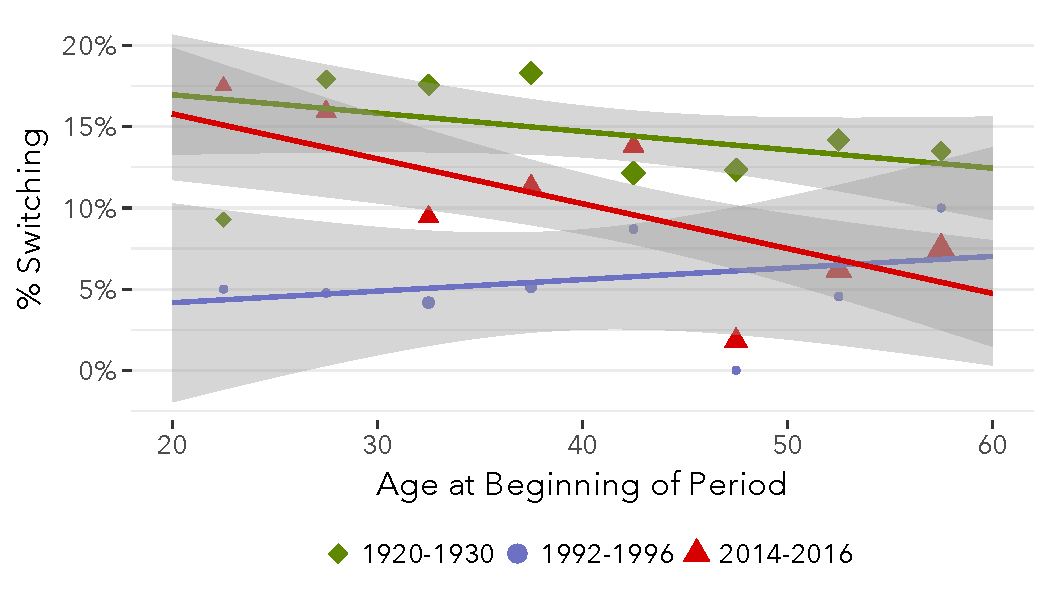
\includegraphics[width=\maxwidth]{figures/plots-switching_by_age-1} 

}

\caption[Rates of party switching by age for three different sets of panel data]{Rates of party switching by age for three different sets of panel data. The 2014-2016 rates are weighted according to the ATP panel weights. Each solid line shows a bivariate linear regression fit to the data, with a 95\% confidence interval shown in grey. The circumscribed area of the symbols is proportional to the number of people represented by each point.}\label{fig:switching_by_age}
\end{figure}


\end{knitrout}
% 
% 
% %\subsection*{Voting in Groups}
% 
% Social identities may provide a clue as to why partisanship became more stable after the realignment. In the 1910s and 1920s, major demographic categories related to class, national origin, age and gender had no partisan valence: every demographic group was similarly majority-Republican \citep{spahn2018before}. In modern times, partisan differences exist along all of these dimensions, strengthening individuals' ties to their party \citep{mason2016cross} and insulating them from cross-cutting pressures. Partisan class differences emerged sharply during the realignment, aligning identity, policy interests and party attachments. It is impossible to causally tie the emergence of class cleavages with the emergence of partisan stability, but the fact that the two emerged in tandem is highly suggestive of the mechanism in play.
% 
% 
% The observation that public opinion is driven by group identities is not new, but it has received new attention recently, as Achen \& Bartels \citeyearpar{achen2016democracy} have argued that group identities are the best framwwork with which to understand individuals' political choices.  This is surely a useful framework for thinking about the present, but the social groupings of the pre-Realignment era did much less explanatory work before the New Deal.
% 
% %\subsection*{Class}
% 
% % footnote about women
% % white collars also realign
% 
% The coalescing of the American party system around competition between parties representing the interests of capital (the Republicans) labor (the Democrats) is one of the defining facts of the New Deal Realignment. Lipset \& Rokkan \citeyearpar{lipset1967cleavage} document this trend in several Western countries, observing that the social divisions of the 1920s were expressed in the agendas of political parties and frozen in place in what appeared to be permanent political divisions. The context for this so-called \textit{freezing hypothesis} is important, as it tells us about the pre-conditions for permanent class cleavages to take hold.  Lipset \& Rokkan's argument applies to advanced democracies broadly, but the American transition from the fourth to the fifth party system can serve as an interesting study of how this freezing took place.
% 
% It might not be mere coincidence that that the freezing of partisan identities  and the freezing of the core cleavage defining the (non-Southern) American party system both occured in 1936.  Before the New Deal realignment, party registration was fluid, so large changes in the issue orientation of the parties could be bolstered by a large pool of loosely attached voters that could rally behind the party's new platform.  This is surely what happened during the New Deal realignment, which led voters from across the social classes to coalesce and solidify behind the Democrats. These voters, once captured by the Democratic party or by the Republicans, stayed, and the issue orientation of the parties solidified.  Would the parties have been able to hold on to their newly-loyal voters if they changed their core platforms? Perhaps so, but in the context of two nationally competitive parties with stable bases, elites that sought to change the orientation of the party could not rely on an influx of new party members to bolster reform against pressure from incumbent members invested in the status quo. In the context of loyal partisans, a change in issue orientation may have been too risky for parties committed to maintaining incumbents' hold on power.




%Before 1932, and particularly before 1918, the relationship between social class and partisanship was remarkably weak. There was virtually no absolute difference in the partisanship of people of different social classes. After at least 22 years of partisan competition not organized along class lines, a class cleavaged emerged rapidly in the New Deal realignment. Thus, even if an individual saw their own class identity as important to their self-conception, this identity wouldn't have a clear partisan valence. In this sense, class identity wouldn't be tied up in politics, and couldn't be used as a defense against cross-pressuring information that might lead a voter to switch parties.








% \subsection*{National Origin}
% 
% 
% In the absence of clear individual-level partisanship data, it is often convenient to discuss partisanship in terms of geographically concentrated groups. Because people of common national origin tend to concentrate geographically and share cultural traditions, it is natural to talk about ethnic groups as salient to political competition. Lubell \citeyearpar{lubell1952future} believed that the influx of immigrants in the early twentieth century had made a large partisan change inevitable. Whether one believes the realignment was destiny, it does not  follow that immmigrants had distinctive political attachments before the realignment.
% 
% Compared to today, when African-Americans and hispanics are substantially more likely to vote for Democrats than  whites, the race and ethnic divisions of the time were small.  In both 1930 and 1940, the partisanship of African-Americans nearly exactly matched that of whites. This suggests that there was no racial cleavage for the black population, which made up around 1.5\% of the state's voters. 
% 
% Among immigrants and their children, there was at best a modest relationship between ethnic origin before the realignment.  Figure~\ref{fig:natl_origin} shows the relationship by father's national origin between parisanship in 1930 and 1940. In 1930, the standard deviation of the two-way Democratic registration share (the horizontal variation) was 6.7\%. After the realignment, this variation (the vertical varation in figure~\ref{fig:natl_origin}) increased by a third, to 9.2\%.  Though there was certainly some variation explained by immigrant group, the variation explained is small.  In 1930, 18\% of Californians with native fathers were Democrats, as were Californians with foreign-born fathers. Indeed, with the exception of a few ethnic groups, most ethnic groups were also near the 18\% average. After the realignment, first and second-generation immigrants were 5 percantage points more Democratic than those with native-born parents. 
% 
% This difference only grew with time. In 2013, second-generation hispanic immigrants were 23 percentage points more Democratic than the American public generally, while Asians were six points more Democratic. Thus, the non-existent nativity gap of the pre-New Deal period is anomolous both by the standards of post-realignment politics and of today.



%The partisanship of immigrants before the New Deal is not merely important as a description of public opinion before the New Deal, it also provides important context for understanding the mobilization account of the realignment. In the mobilization story, much of the increase in Democratic votes during the realignment comes from the mobilization of immigrants and their children. But if the mobilization account is to be believed, these immigrants and their children must already have been Democrats (or disposed to become Democrats) and simply were not voting. We cannot know the party registrations of people that weren't registered to vote, but it stands to reason that those first and second-generation immigrants that were registered to vote were politically similar to those that were not.  If this was the case, then the unregistered population was about as Democratic as those that were registered to vote, making the mobilization account implausible.


\FloatBarrier
\subsection*{Generational Distinctiveness}


The relative responsiveness of young people to political tides has produced a characteristic feature in American public opinion: generational distinctiveness.  Different generations, which came of age during different political climates, tend to have distinctive partisan compositions. Those that came of age during the New Deal, a time when Democrats were overwhelmingly popular, tend to be more supportive of Democrats.  Younger Americans who came of age during the Reagan years, a time of Republican ascendancy, tend to be more supportive of Republicans.

Generational distinctiveness relies on two features of American political behavior: the sensitivity of young people to the political environment and the stability of partisanship after an initial partisan identity is formed.  Though  differences in partisan stability by age have not been directly observed until recently, that people's long-term partisan preferences are most sensitive to the political environment in the years of their teens and early-twenties implies that this must be a period of greater fluidity \citep{ghitza2014great}. After this generational distinctiveness is forged in young adulthood, it is preserved by the stability of partisanship later in life. 

The phenomenon of generational distinctiveness tells us that for the most part, partisan change proceeds through the replacement of one generation with another. As the silent generation declines in their share of the electorate, millennials replace them. Since millennials are 27 percentage points more supportive of Democrats than the silent generation, strict replacement, without any partisan change in either group, represents a large advantage to the Democrats \citep{bonica2018whats}. 

Generational replacement has replaced realignment as the driver of partisan change in America. Despite the partisan instability of today's electorate, broad-scale partisan change, of the kind seen during the New Deal realignment, is unlikely to occur because the present instability is concentrated among the youngest voters. Older voters, who have had longer to be socialized into a particular political party, hold on to their partisanship at similar rates to the period after the New Deal. In contrast, the instability at the beginning of the twentieth-century was broad-based, consistent with an electorate that has not been socialized into supporting one party or the other. In some sense, this means that the whole electorate was more open to change, whereas now, this openness is concentrated among the young. In the absense of partisan socialization, dramatic events like the Great Depression and the New Deal are able to reshape the whole electorate. But in today's era of strong partisanship, these events primarily affect the youngest voters.

Before the realignment, there was virtually no variation in the partisanship of different age groups in California. In both 1920 and 1930, voters of all ages registered with one of the major parties registered with the Democrats about 20\% of the time.  Following the realignment, party switching rates dropped overall and there ceased to be any meaningful variation in party switching by age group. Relative to today, when generational differences in partisanship are a prominent feature of American public opinion, no such differences were present in pre-realignment California \citep{bartels2014generational}. 



\begin{knitrout}
\definecolor{shadecolor}{rgb}{0.969, 0.969, 0.969}\color{fgcolor}\begin{figure}

{\centering 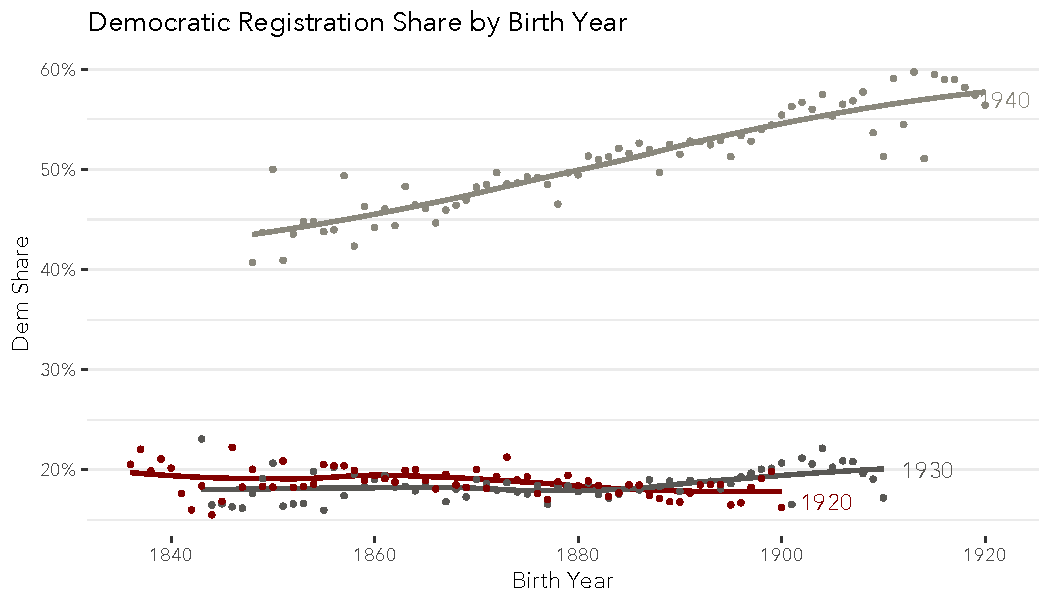
\includegraphics[width=\maxwidth]{figures/plots-age-1} 

}

\caption[Rates of Democratic partisan identification by age]{Rates of Democratic partisan identification by age. For the twentieth-century data, age is drawn from the 1920 and 1930 censuses, matched to the Great Registers of the same year with exact matching on name and street. The 2014 data comes from wave 1 of the Pew American trends panel. The lines represent loess fits to the aggregated data.}\label{fig:age}
\end{figure}


\end{knitrout}



\subsection*{Conclusion}

% move from flip-flop to stable
% 

The tools of public opinion research were developed in an age of structured and stable party affiliations. But before the realignment, mass partisanship was descriptively quite different. 10\% of voters switched parties every four years, a rate of party-switching that was higher than post-realignment levels across demograpic groups. This distinct period of political history occured just before the New Deal realignment, perhaps the most consequential time for mass politics in the twentieth century. Understanding the period from 1908 to 1928 sheds new light on the realignment and helps contextualize the differing accounts of how the realignment took place. In light of what we know about the high rates of partisan fluidity in the pre-realignment period, mass partisan conversion of Republicans into Democrats seems like a more plausible reasoanble account of how the realignment took place.

 Social identities may provide a clue as to why partisanship became more stable after the realignment. In the 1910s and 1920s, major demographic categories related to class, national origin, age and gender had no partisan valence: every demographic group was similarly majority-Republican \citep{spahn2018before}. In modern times, partisan differences exist along all of these dimensions, strengthening individuals' ties to their party and insulating them from cross-cutting pressures \citep{mason2016cross}. Partisan class differences emerged sharply during the realignment, aligning identity, policy interests and party attachments. It is impossible to causally tie the emergence of class cleavages with the emergence of partisan stability, but the fact that the two emerged in tandem is highly suggestive of the mechanism in play.
% 
% 
 The observation that public opinion is driven by group identities is not new, but it has received new attention recently, as Achen \& Bartels \citeyearpar{achen2016democracy} have argued that group identities are the best framwwork with which to understand individuals' political choices.  This is surely a useful framework for thinking about the present, but the social groupings of the pre-Realignment era did much less explanatory work before the New Deal.
% 

The pervasiveness of party-switching before the realignment might also explain the longevity of the post-New Deal party system. If the New Deal realignment was facilitated by weak and fluid partisan attachments in the period that preceded it, any realignment occuring later would not benefit from these same fluid attachments.  There are some indications, however, that partisan fluidity is increasing.  Recent panel data from the Pew Research Center \citeyearpar{doherty2017partisan} has shown an uptick in party-switching rates, with 10\% of partisans changing parties from 2015-2016. This rate of party-switching is higher than has been observed in any period of stable partisanship since the advent of modern polling, but it has been occuring for a relatively short period. The pre-realignment fludity persisted for at least twenty years.

That the distinctive character of politics before the realignment went undiscovered for nearly 90 years is no surprise; the research tools to conduct this analysis simply did not exist. To understand how difficult it is for humans unaided by computers to work with voter list data, it helps to draw an analogue with turnout validation. In the early years of the ANES, respondents' self-reported turnout was validated against county voting records, but this validation was eventually abandoned as it was too difficult for interviewers. To produce a panel analysis of the Great Registers without the benefit of contemporary optical-character recognition and data-management software, research assistants would have to cross-reference individual voters within bound voter lists, later finding these same voters in paper census records. It's hard to estimate how proficient research assistants could be trained for this task, but the benefits of modern technology are clear.  To study this period before surveys, computing power tied to suitable administrative records is the only viable means of gathering individual data.

These records overturn many would-be laws of American public opinion. Research on realignments conceives of partisanship as generally static, punctuated by periods of rapid change. But before the New Deal, individual change was constant, even as macropolitics were in a stable Republican-dominated equilibrium. When the earliest entries into the canon of American political behavior were written in the 1950s, America had enjoyed a relatively stable two decades of partisan competition. Voters had stable party affiliations that flowed in part from their membership in social groups. Had the survey-based architecture of American public opinion formed twenty years earlier, very different accounts of American political behavior would have been written. Partisan stability would be treated not as an essential element of the American political mind, but instead as a historically contingent phenomenon emerging out of the tumult of the 1930s. Given the picture of partisanship offered by the Great Registers, we now know that the cast of \textit{The American Voter} was forged in 1936.




\clearpage
\bibliographystyle{apsr}
\bibliography{realignment}

\appendix


\FloatBarrier
\newpage
\section*{Appendix}
\subsection*{Is California a representative case?}

Even if one accepts that the Great Registers provide a reasonable picture of Californians' partisan attachments, the connection between California politics and those of America broadly is up for debate. Even in 1910, California was home to nearly 2.4 million people, a population that more than quadrupled by 1950. The political behavior of these Americans should itself be of interest.  But if these Californians are reasonable proxies for the behavior of their eastern compatriots, a broader and more important story can be told.  


Counties are the lowest geographic unit for which election data is consistently available for the early twentieth century; at this level voting in California looked broadly similar to the rest of the non-Southern states.  Figure~\ref{fig:countydensity} shows the distribution of county-level presidential vote for 1912-1940 in California and in other non-Southern states. Except in 1924, when Progressive presidential candidate Robert La Folette was popular among historically-Democratic rural voters in California, the distribution of county-level Democratic presidential vote was near the median of the distribution of the same measure in non-Southern states. One other way that California is unrepresentative is that in 1912, Taft did not appear on the ballot. Instead, voters chose between Wilson, running as a Democrat and Theodore Roosevelt, running under the Progressive banner.

Returning to the Literary Digest polls discussed in the introduction, we can evaluate not just presidential vote, but vote-switching. Californians had rates of political defection about as high as voters in non-Southern states overall. Among Californians, 52\% of Davis voters switched to Hoover in 1928, while 26\% switched from Coolidge to Smith.  The comparable national numbers were 35\% and 23\%, respectively. The rate of defection among Californians is higher than among voters nation-wide, but both shared a rate of vote-switching much higher than typical in modern elections.




\begin{knitrout}
\definecolor{shadecolor}{rgb}{0.969, 0.969, 0.969}\color{fgcolor}\begin{figure}

{\centering 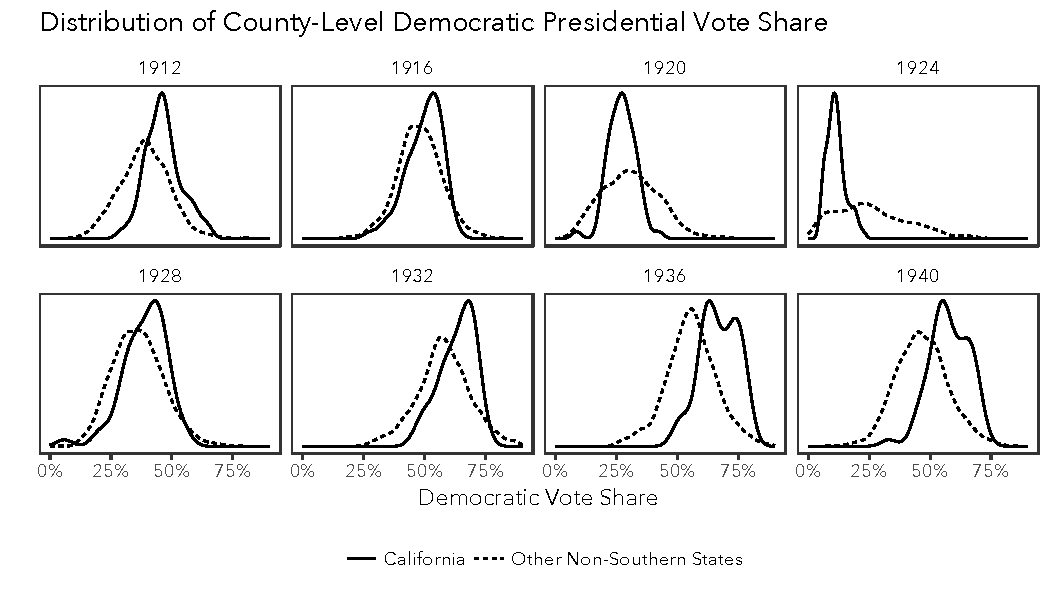
\includegraphics[width=\maxwidth]{figures/plots-countydensity-1} 

}

\caption[Density plots of county-level presidential vote share for California (the solid line) and counties in non-Southern states (dashed line) for presidential elections 1912-1940]{Density plots of county-level presidential vote share for California (the solid line) and counties in non-Southern states (dashed line) for presidential elections 1912-1940. For the purposes of this analysis, Alabama,	Arkansas,	Florida,	Georgia,	Kentucky,	Louisiana,	Mississippi,	North Carolina,	South Carolina,	Tennessee,	Texas,	Virginia and	West Virginia were removed.}\label{fig:countydensity}
\end{figure}


\end{knitrout}

%Another possible source of difference is in polarization. Masket (YEAR)
\FloatBarrier

\subsection*{Is party registration a substitute for party affilation?}

% Jerry Ruske talks about how voting is more intense
% Keller, Morton. Affairs of State: Public Life in Late Nineteenth Century America (1977)


Papers on partisan dynamics in public opinion usually rely on some version of the party affiliation question first developed by George Gallup in the 1930s \citep{clarke2009dynamics}. Because the question wasn't invented until after the realignment, party registration from the Great Registers will have to suffice. Luckily, the county-level two-party Democratic registration rate from the Great Registers and the county-level two-party presidential vote have a correlation of .7, indicating that they both pick up on a latent quality of voters, partisanship. To the extent that there is a divergence between the two measures, the registration rate is less variable, as shown in figure~\ref{fig:countyparty}. This is in line with our conception of party affiliation as being more stable than presidential vote choice, which includes a component that reacts to the particulars of the candidate, rather than the party, which is by its nature more stable.

One other explanation for the slow change in partisanship is that voters' choice of party is simply out of line with their actual party affiliation, with registrations reflecting a habit of registering with the same party year-after-year rather than actual partisan feeling.  Fortunately, the rapid increase in the Democratic registration rate from 1930 to 1936 along with the increase in the Democratic vote share, both in California and nationally, suggests that when party allegiances truly do shift in the aggregate, as we know happened during the New Deal realignment, Californians' party registration followed suit. Figure~\ref{fig:countyparty} shows that from 1928-1936, when the New Deal realignment dramatically increased the level of support for Democratic candidates, Democratic party registration also increased dramatically.


Finally, many descriptive facts about partisanship learned after the New Deal are actually reflected in the data. After the realignment, partisanship is stable, blue-collar workers are more aligned with the Democratic party than white-collar workers, and younger voters are more likely to be Democrats than older voters, which aligns with other research about the post New-Deal period \citep{campbell1960american,alford1963role}. That these structural features of the post-New Deal party system, gleaned from election returns and surveys, also aligns with this California voter registration data should give us further confidence that this data will give us valid inferences about politics before the New deal.

% Talk more about tighter correlation post-realignment

\begin{knitrout}
\definecolor{shadecolor}{rgb}{0.969, 0.969, 0.969}\color{fgcolor}\begin{figure}

{\centering 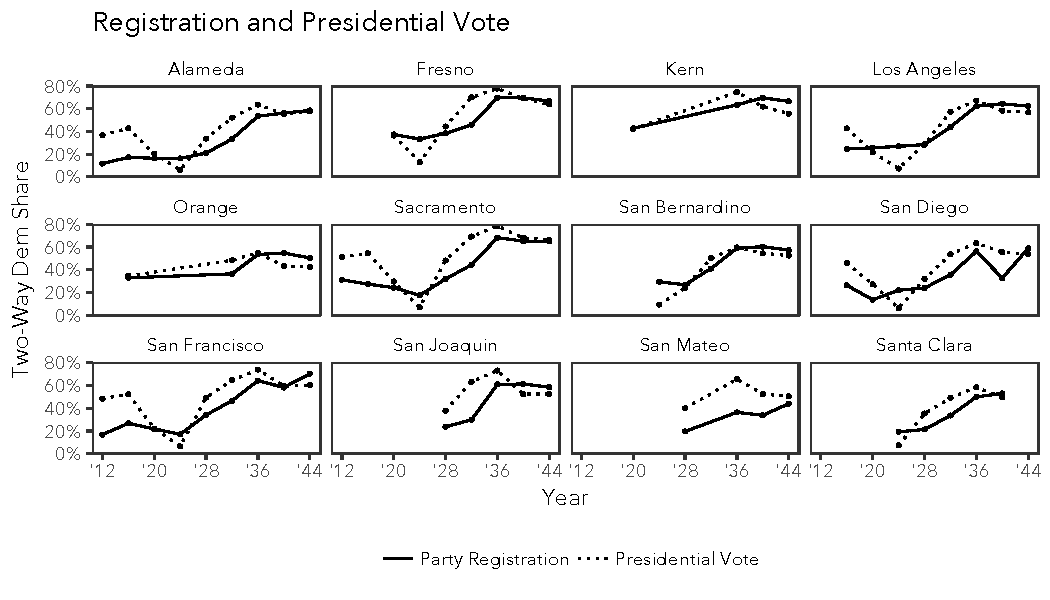
\includegraphics[width=\maxwidth]{figures/plots-countyparty-1} 

}

\caption[Two-Way Democratic presidential vote share and Two-Way Democratic Registration share by year]{Two-Way Democratic presidential vote share and Two-Way Democratic Registration share by year. Due to issues extracting data from the Great Registers, not every county has registration data for every year. For clarity, when data from the Great Registers is missing, data on presidential vote for that county-year pair is also excluded. Only counties that had Great Register data before 1930 and after 1936 were included in this plot.}\label{fig:countyparty}
\end{figure}


\end{knitrout}


\FloatBarrier
\subsection*{Suggestive Evidence of instability}

Some hints of the distinctive political nature of the pre-realignment period have appeared in the literature.  Walter Dean Burnham \citeyearpar{burnham1965changing}, describing the changes in American politics of the first sixty years of the twentieth century, noted that the 1920s featured unusually large variation in partisan vote shares up and down the ballot.  This gap, which he uses as a measure of split-ticket voting, suggests that voters felt less tied to voting for a particular party, casting some votes for one party and some for another. Using aggregated data to infer individual political behavior is fraught, but the result should at least be suggestive that party attachments were weaker during the period.

A better way to learn about individual behavior is with individual-level data.  Drawing on the 1928 Literary Digest poll, Eriksen \& Tedin \citeyearpar{erikson1981partisan} show that 26\% of respondents voted for one of the two major parties in the 1924 election, only to vote for the other party's candidate four years later. A similar pattern appears in the 1916 Literary Digest Straw Poll, which consisted of an opt-in sample covering five contested states. 15\% of Hughes (Rep) voters in 1916 reported voting for Wilson (Dem) in 1912 while 30\% of Wilson voters in 1916 voted for Taft (Rep) or Roosevelt (Prog) in 1912.\footnote{Wilson won the 1912 election in part because Taft and Roosevelt split the Republican vote, allowing Wilson to win with 42\% of the total. Because there were two Republican-aligned candidates, the rate of Republican and Progressive voters from 1912 voting for Wilson in 1916 is probably higher than if only one had run, thereby increasing the defection rate overall.} Again, the overall high rate of defection, 20\%, is obscured by the smaller net shift of 8\% towards Wilson between 1912 and 1916.  

The rates of defection for 1912-1916 and 1924-1928 were appreciably higher than the defection rates of 17\% for 1936-1940 and 11\% for 1940-1944 \citep{erikson1981partisan,key1966responsible}. The disparity in defection rates before and after the New Deal realignment suggests that a paradigm shift took place, not just in the partisanship of voters, but also in the degree to which voters were attached to their party.

The evidence from the Literary Digest Straw Polls is certainly suggestive of a change, but their value is limited by their opt-in design, which produced biased samples \citep{squire19881936}. The polls also didn't ask demographic questions that might help explain who is changing their votes. Finally, the Straw Poll didn't ask for the respondent's party affiliation, an essential piece of information to understand a voter's political leanings independent of their preferences for a particular candidate \citep{campbell1960american}. Taken together, the drop off in vote-switching between the pre-realignment Literary Digest polls and the post-realignment Gallup polls suggests that American political behavior before the realignment was characterized by weaker party attachments, but the evidence is hardly conclusive. To throw out the conventional account of the party-driven American voter for the pre-realignment period, more individual-level evidence of partisan change is needed. 


\subsection*{The Registers Show Stability After 1936}

Survey data collected after the New Deal realignment suggests that we should see a low level of inter-party defections after the New Deal. This pattern is unambiguous in the Great Registers, only about 2.5\% of registrants change their party registration from one presidential election to the next. The correspondence between these results shows that behaviors observed on the Great Registers match survey results, thereby increasing the credibility of the Great Registers as a research tool. It also makes the volatility of the pre-realignment period more striking; the volatility of the first three decades of the twentieth century is totally out of line with the partisan stability of the post-realignment period.

The passage of Proposition 14 in 1930 changes the interpretation of the post-1932 data. The measure amended the statute governing voter registration, requiring the state to maintain registrations from the previous two-year election cycle and allow the previous cycle's voters to vote in the next cycle without re-registering. This meant that voters that voted consistently would not  need to file a new registration nor update their occupation or party registration. Non-voters, however, would be removed from the rolls and sent a postcard alerting them that they had to re-register to vote in the next election. About 20\% of registered voters didn't vote in presidential general elections and 25-40\% didn't vote in midterms, so many voters did have to file new registrations each year, in addition to those that had to re-register due to a change in residence. 

These re-registrants are key to creating a set of voters who made updates to their voter registration, just as all registrants did before 1934. Among the set of registrants matched to their own registration from four years later in figure~\ref{fig:pid_switching}, I want to identify those that were not registered in the midterm election, indicating that they had to re-register in advance of the next presidential election. The matching method used for the figure~\ref{fig:pid_switching} panel was quite conservative, only making matches when the match was nearly certain. This restriction surely missed many correct matches, but it kept the false positive rate to a minumum, thereby minimizing the bias toward a higher rate of defections created by erroneous matches. To identify registrants missing from the midterm election rolls, a more relaxed match method is necessary. Such a match method should, to the extent possible, minimize the false negative rate, so that panelists that might not have had to re-register can be excluded.  The goal is to find a subset of panelists that would have had to re-register.

To perform this matching, I used fastlink to identify Presidential-year records that had at least one record in the following midterm year matched by \emph{fastlink} with a probability  greater than $.2$. Presidential-year records in the quadrennial panel for which at least one matching midterm record was found are marked as continuous registrations while cases where no midterm record was found are marked as new. Before the rule change, 73\% of registrations are marked as continuing, while after the change, 89\% of registrations are marked as continuing, suggesting that the rule change had the intended effect of maintaining more registrations.\footnote{The test for equality of proportions is significant at the $p \approx 0$ level. Using just the elections immediately before and after the change, the continuous registration rate increased from 73\% to 84\%, which is also significant at the  $p \approx 0$ level. } On average, each continuous registration case was matched to 6 midterm cases, which suggests that the false positive rate for the matching procedure was extremely high. This surely mis-classified many voters as continuous registrants, but increases the confidence that any registration marked as new was indeed attached to a voter that had to re-register for that election.

The party switching rates for new and continuing registrations are plotted in figure~\ref{fig:prop14}. Among the 10\% of presidential-election registrants for which no midterm registration appeared, the party-switching rate averaged just 3\% and never exceeded 5\%, indicating that party-switching had indeed fallen from the 10\% rate observed before the realignment. If indeed the fall in party-switching rates was merely an artifact of the rule-change, rather than a genuine change in political behavior, the party-switching rate for new registrations would be around 10\%, as it was before the realignment.


\begin{knitrout}
\definecolor{shadecolor}{rgb}{0.969, 0.969, 0.969}\color{fgcolor}\begin{figure}

{\centering 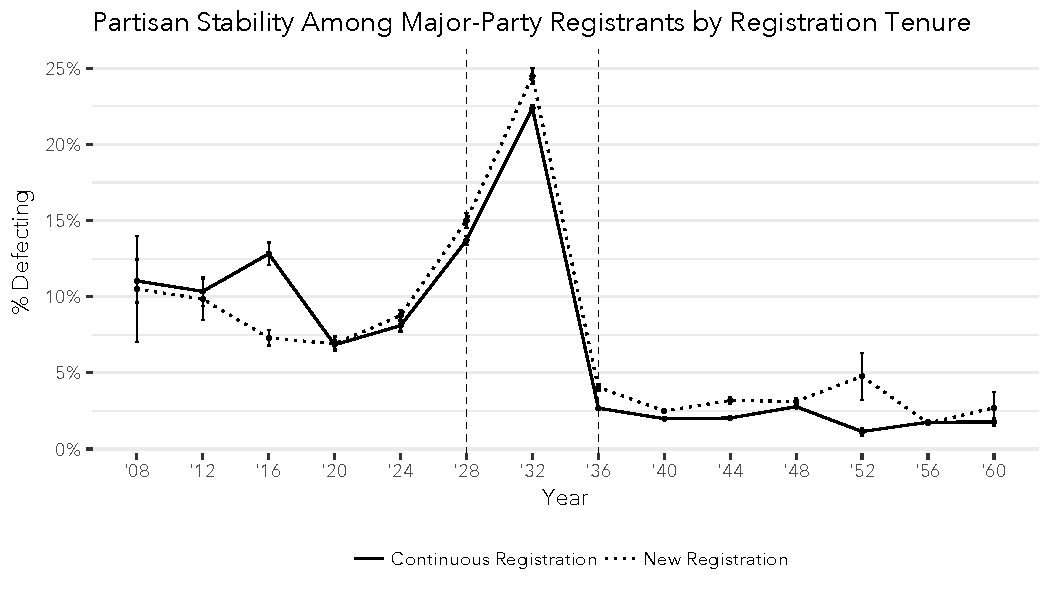
\includegraphics[width=\maxwidth]{figures/plots-prop14-1} 

}

\caption[Rates of party switching between successive presidential elections among voters registered with the two major parties in both elections]{Rates of party switching between successive presidential elections among voters registered with the two major parties in both elections. The figure was generated by matching records appearing in successive presidential years that share an address, surname, and first name (using the corrected first and last names discussed earlier). Records for which no registration in the midterm election was found are classified as having a new registration, while voters that were registered in the midterm are classified as having a continuous registration. For the purposes of matching a midterm registration, a loose match method was used, leading to many new registrations to be falsely classified as continuing. Frequentist 95\% confidence intervals are plotted as vertical lines.}\label{fig:prop14}
\end{figure}


\end{knitrout}

    \end{document}
    
